\documentclass[t]{beamer}

\usetheme{Air}
\usepackage{graphics}
\usepackage{graphicx}
\graphicspath{{C:/Users/Brayden/Projects/PEPS-Data/}{.}}
%\usepackage{caption}
\usepackage{amsthm}
%\usepackage{thumbpdf}
\usepackage{wasysym}
\usepackage{ucs}
\usepackage[utf8]{inputenc}
\usepackage{pgf}
\usepackage{verbatim}
\usepackage{tikz}
\usepackage{pgfmath}
\usetikzlibrary{calc}
\usetikzlibrary{backgrounds}
\usetikzlibrary{arrows}
\usetikzlibrary{shapes.arrows}
\usetikzlibrary{shapes.geometric}
\usetikzlibrary{decorations.markings}
\usetikzlibrary{positioning}
\usetikzlibrary{fit,chains}
\usepackage{natbib}
\usepackage{wasysym}
\usepackage{soul} 
\bibliographystyle{apalike}  

%\usepackage{pstricks}
%\newpsobject{psid}{psline}{linestyle=dotted,dotsep=1pt}
%\newpsobject{pspsi}{psline}{doubleline=true}
%\newpsobject{pssigma}{psline}{linewidth=1.5pt}

%\usepackage{pgfpages}
%\setbeamertemplate{note page}[plain]
%\setbeameroption{show notes on second screen=right}
%http://tex.stackexchange.com/questions/21777/is-there-a-nice-solution-to-get-a-presenter-mode-for-latex-presentations

\newcommand{\beq}{\begin{equation}}
\newcommand{\eeq}{\end{equation}}
\newcommand{\beqa}{\begin{eqnarray}}
\newcommand{\eeqa}{\end{eqnarray}}
\newcommand{\bi}{\begin{itemize}}
\newcommand{\ei}{\end{itemize}}
\newcommand{\ket} [1] {\vert #1 \rangle}
\newcommand{\bra} [1] {\langle #1 \vert}
\newcommand{\braket}[2]{\langle #1 | #2 \rangle}
\newcommand{\ev}[1]{\langle #1 \rangle}
\newcommand{\vbra}[1]{\left ( #1 \right |}
\newcommand{\vket}[1]{\left |#1 \right )}
\newcommand{\vbraket}[2]{\left ( #1 \middle |#2 \right )} 
\newcommand{\braopket}[3]{\left \langle #1 \middle |#2 \middle | #3 \right \rangle} 
\newcommand{\vbraopket}[3]{\left ( #1 \middle |#2 \middle | #3 \right )} 

%\newcommand<>{\highlighton}[1]{%
%  \alt#2{\structure{#1}}{{#1}}
%}

\newcommand{\icon}[1]{\pgfimage[height=1em]{#1}}

\tikzset{peps/.style={circle=2pt,draw=black!100,fill=green!50,inner sep=3pt}}
\tikzset{bpeps/.style={circle=2pt,draw=black!100,thick,fill=green!50,inner sep=3pt}}
\tikzset{gamma/.style={circle=2pt,draw=black!100,fill=blue!20,inner sep=3pt}}
\tikzset{lambda/.style={rectangle,rotate=45,draw=black!100,fill=orange!50,inner sep=4pt}}
\tikzset{operator/.style={circle=2pt,draw=black!100,fill=orange!80,inner sep=3pt}}
\tikzset{cdot/.style={circle=2pt,draw=black!100,fill=white,inner sep=1pt}}
\tikzset{bg/.style={rounded corners,thin,fill=blue!10}}
\tikzset{inv/.style={opacity=0}}
\tikzset{spin/.style={circle=2pt,draw=black!100,fill=orange!80,inner sep=3pt}}
\tikzset{unitbox/.style={fill=black!3,rounded corners}}
\tikzset{corner/.style={rectangle=10pt,fill=blue!50,draw=black}}
\tikzset{side/.style={rectangle=6pt,fill=blue!20,draw=black}}
\tikzset{cside/.style={circle=6pt,fill=blue!20,draw=black}}
\tikzset{swapg/.style={circle=1pt,draw=black,fill=black!80,inner sep=1pt}}

\tikzset{base/.style={circle=2pt,fill=orange!80,draw=black}}
\tikzset{det/.style={circle=2pt,fill=blue!20,draw=black,inner sep=4pt}}
\tikzset{iso/.style={circle=2pt,fill=red!20,draw=black,inner sep=4pt}}
\tikzset{top/.style={circle=2pt,fill=black!20,draw=black,inner sep=4pt}}
\tikzset{siso/.style={circle=1pt,fill=red!20,draw=black,inner sep=1pt}}

%Brayden's
\tikzset{GHZ/.style={circle=2pt,fill=black!80,draw=black,inner sep=2pt}}
\tikzset{X/.style={circle=2pt,fill=black!80,text=white,font=\footnotesize, draw=black,inner sep=1pt}}
\tikzset{W/.style={circle=2pt,fill=black!20,draw=black,double,inner sep=2pt}}
\tikzset{eli/.style={ellipse, rotate=0, draw=black, fill=gray!20}}

%http://tex.stackexchange.com/questions/199683/how-to-plot-quantum-logical-gates-with-tikz
\tikzset{
cross/.style={path picture={ 
            \draw[thick,black](path picture bounding box.north) -- (path picture bounding                  box.south) (path picture bounding box.west) -- (path picture bounding                      box.east);
            }},
crossx/.style={path picture={ 
            \draw[thick,black,inner sep=0pt]
                (path picture bounding box.south east) -- (path picture bounding box.north west) (path picture bounding box.south west) -- (path picture bounding box.north east);
            }},
circlewc/.style={circle=2pt,draw, crossx}
}
%\newtheorem{LSM}{{\em Theorem: Lieb, Schultz, Mattis (1961)}}
%\newtheorem{Oshikawa}{{\em Extension: Oshikawa (1999)}}

\pdfinfo
{
  /Title       (bd)
  /Creator     (TeX)
  /Author      (Brayden Ware)
}


\title{Brayden's Diagrams}
%\subtitle{}
\author{Brayden Ware}
\date{September 30th 2014}

\begin{document}

\frame{\titlepage}


%%%%%%%%%%%%%%%%%%%%%%%%%%%%%%%%%%%%%%%%%
%%%%%%%%%% Pre-outline section %%%%%%%%%%
%%%%%%%%%%%%%%%%%%%%%%%%%%%%%%%%%%%%%%%%%
% \section*{}

% \begin{frame}{Frame Title}
\vskip-1.5cm

\end{frame}

%%%%%%%%%%%%%%%%%%%%%%%%%%%%%%%%%%%%%%%%%
%%%%%%%%%% Outline code %%%%%%%%%%%%%%%%%
%%%%%%%%%%%%%%%%%%%%%%%%%%%%%%%%%%%%%%%%%
\section*{}

\begin{frame}
  \frametitle{Outline}
  \vskip-1.5cm
  \tableofcontents
\end{frame}

\AtBeginSection[]
{
\frame{
  \vspace{2cm}
  {\huge \insertsection}
  }
}
%\AtBeginSection[]
%{
%  \frame<handout:0>
%  {
%    \frametitle{Outline}
%    \vskip-1.5cm
%    \tableofcontents[currentsection]
%  }
%}

%\AtBeginSubsection[]
%{
%  \frame<handout:0>
%  {
%    \frametitle{Outline}
%    \tableofcontents[sectionstyle=show/hide,subsectionstyle=show/shaded/hide]
%  }
%}
%%%%%%%%%%%%%%%%%%%%%%%%%%%%%%%%%%%%%%%%%
%%%%%%%%%% Content starts here %%%%%%%%%%
%%%%%%%%%%%%%%%%%%%%%%%%%%%%%%%%%%%%%%%%%

\section{Diagrams}
\begin{frame}
\scalebox{1}{
\begin{frame}{MPS Example: AKLT State}
\vskip-1.5cm
\begin{block}{Haldane Phase for Spin-1 chains $(j=1, m=0)$}
\vskip-0.8cm
$$
H_{AKLT} = \sum\limits_{i} J \vec{S}_i\cdot \vec{S}_{i+1} + J' (\vec{S}_i\cdot \vec{S}_{i+1})^2 + D (S^z_i)^2+BS^x
$$
\end{block}
\begin{columns}[T]
    \begin{column}[T]{.45\textwidth}
        \vskip-1.2cm
        \begin{figure}
        \centering
        \includegraphics[width=\columnwidth]{diagrams/aklt2.png}
        \end{figure}
    \end{column}
    \begin{column}[T]{.55\textwidth}
    \vskip-0.8cm
    Two distinct featureless insulators:
    \bi 
    \item Large-D phase
    \bi 
    \item Contains product state wavefunction $\ket{\psi} = \ket{000...}$ 
    \ei
    \item Haldane phase
    \bi 
    \item Contains AKLT wavefunction $\ket{\psi} = \Sigma\ket{+00-0+...}$
    \ei 
        \begin{figure}[h]
            \hspace{-2cm}
            \scalebox{1.2}{
            \begin{frame}{MPS Example: AKLT State}
\vskip-1.5cm
\begin{block}{Haldane Phase for Spin-1 chains $(j=1, m=0)$}
\vskip-0.8cm
$$
H_{AKLT} = \sum\limits_{i} J \vec{S}_i\cdot \vec{S}_{i+1} + J' (\vec{S}_i\cdot \vec{S}_{i+1})^2 + D (S^z_i)^2+BS^x
$$
\end{block}
\begin{columns}[T]
    \begin{column}[T]{.45\textwidth}
        \vskip-1.2cm
        \begin{figure}
        \centering
        \includegraphics[width=\columnwidth]{diagrams/aklt2.png}
        \end{figure}
    \end{column}
    \begin{column}[T]{.55\textwidth}
    \vskip-0.8cm
    Two distinct featureless insulators:
    \bi 
    \item Large-D phase
    \bi 
    \item Contains product state wavefunction $\ket{\psi} = \ket{000...}$ 
    \ei
    \item Haldane phase
    \bi 
    \item Contains AKLT wavefunction $\ket{\psi} = \Sigma\ket{+00-0+...}$
    \ei 
        \begin{figure}[h]
            \hspace{-2cm}
            \scalebox{1.2}{
            \begin{frame}{MPS Example: AKLT State}
\vskip-1.5cm
\begin{block}{Haldane Phase for Spin-1 chains $(j=1, m=0)$}
\vskip-0.8cm
$$
H_{AKLT} = \sum\limits_{i} J \vec{S}_i\cdot \vec{S}_{i+1} + J' (\vec{S}_i\cdot \vec{S}_{i+1})^2 + D (S^z_i)^2+BS^x
$$
\end{block}
\begin{columns}[T]
    \begin{column}[T]{.45\textwidth}
        \vskip-1.2cm
        \begin{figure}
        \centering
        \includegraphics[width=\columnwidth]{diagrams/aklt2.png}
        \end{figure}
    \end{column}
    \begin{column}[T]{.55\textwidth}
    \vskip-0.8cm
    Two distinct featureless insulators:
    \bi 
    \item Large-D phase
    \bi 
    \item Contains product state wavefunction $\ket{\psi} = \ket{000...}$ 
    \ei
    \item Haldane phase
    \bi 
    \item Contains AKLT wavefunction $\ket{\psi} = \Sigma\ket{+00-0+...}$
    \ei 
        \begin{figure}[h]
            \hspace{-2cm}
            \scalebox{1.2}{
            \input{diagrams/aklt.tex}
            }
        \end{figure}

    \ei
    \end{column}
\end{columns}

\end{frame}
            }
        \end{figure}

    \ei
    \end{column}
\end{columns}

\end{frame}
            }
        \end{figure}

    \ei
    \end{column}
\end{columns}

\end{frame}}
\end{frame}

\begin{frame}
\scalebox{1}{
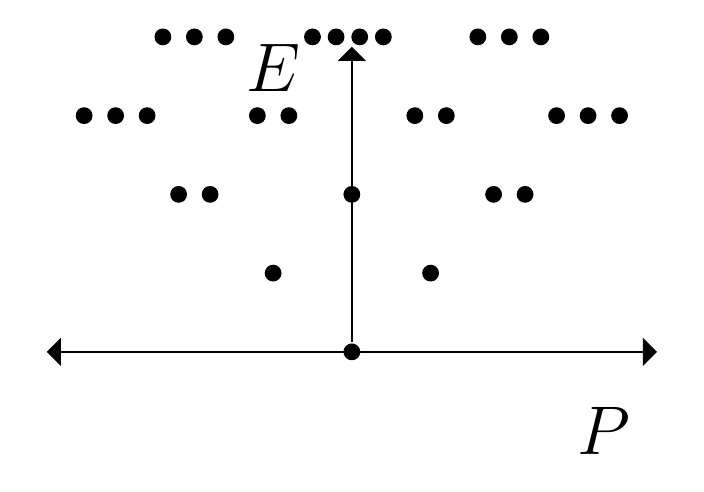
\begin{tikzpicture}
\tikzstyle{yaxis} = [-triangle 90]
\tikzstyle{xaxis} = [triangle 90-triangle 90]
\node[inv](A) at (-4, 0){};
\node[inv](B) at (4, 0){};
\draw[thick, xaxis] (A)-- (B);
\node at ($ (A) !.9! (B) +(0, -1)$) {\Huge $P$};
\node[inv](A) at (0, 0){};
\node[inv](B) at (0, 4){};
\draw[thick, yaxis] (A)--(B);
\node at ($ (A) !.9! (B) +(-1, 0)$) {\Huge $E$};

\tikzset{spec/.style={circle=2pt,draw=black!100,fill=black!100,inner sep=2pt}}
\node[spec] at (0, 0){};
\node[spec] at (1, 1){};
\node[spec] at (1.8, 2){};
\node[spec] at (2.2, 2){};

\node[spec] at (2.6, 3){};
\node[spec] at (3.0, 3){};
\node[spec] at (3.4, 3){};

\node[spec] at (0-1, 0+1){};
\node[spec] at (1-1, 1+1){};
\node[spec] at (1.8-1, 2+1){};
\node[spec] at (2.2-1, 2+1){};

\node[spec] at (2.6-1, 3+1){};
\node[spec] at (3.0-1, 3+1){};
\node[spec] at (3.4-1, 3+1){};

\node[spec] at (0-2.2, 0+2){};
\node[spec] at (1-2.2, 1+2){};
\node[spec] at (1.8-2.3, 2+2){};
\node[spec] at (2.2-2.1, 2+2){};

\node[spec] at (0-1.8, 0+2){};
\node[spec] at (1-1.8, 1+2){};
\node[spec] at (1.8-2, 2+2){};
\node[spec] at (2.2-1.8, 2+2){};

\node[spec] at (-2.6, 3){};
\node[spec] at (-3.0, 3){};
\node[spec] at (-3.4, 3){};

\node[spec] at (-2.6+1, 4){};
\node[spec] at (-3.0+1, 4){};
\node[spec] at (-3.4+1, 4){};


\end{tikzpicture}}
\end{frame}

\begin{frame}
\scalebox{0.5}{
%same as 3 but with a box and labels to match

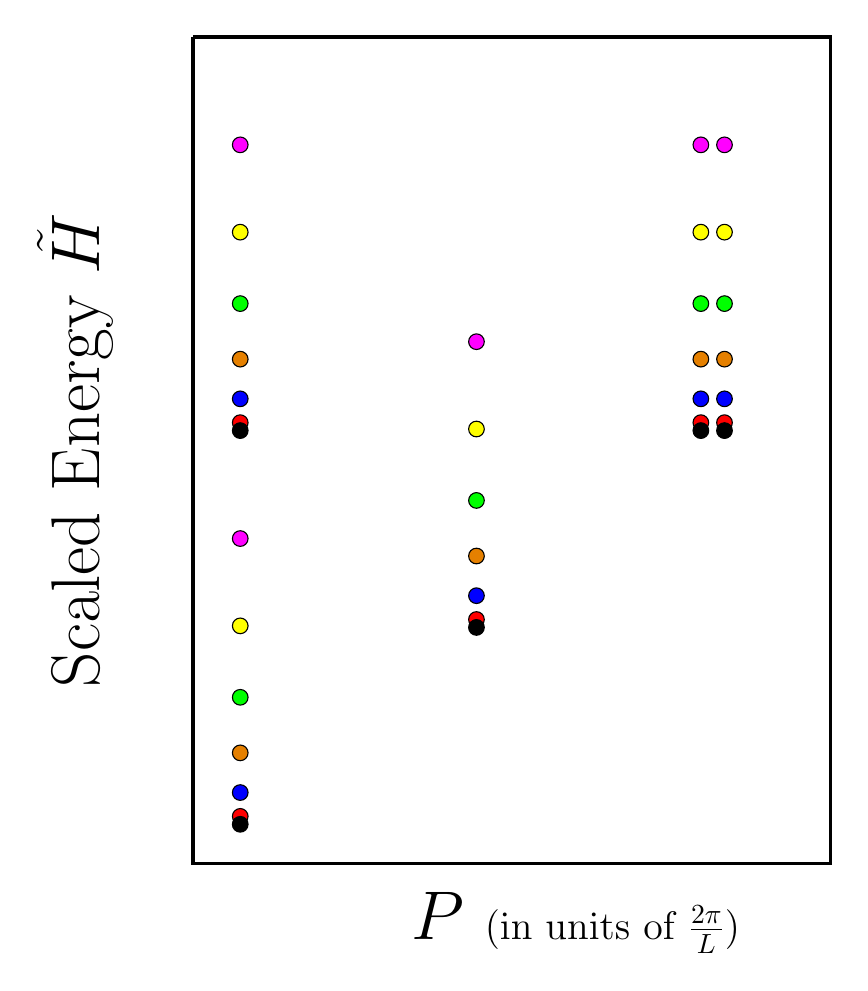
\begin{tikzpicture}[x=30mm,y=25mm]
%\tikzstyle{yaxis} = [-triangle 90]
%\tikzstyle{xaxis} = [triangle 90-triangle 90]
\node[inv](A) at (-.2, -0.2){};
\node[inv](B) at (2.5, -0.2){};
\node[inv](C) at (-.2, 4){};
\node[inv](D) at (2.5, 4){};
\draw[very thick] (C.center)--(A.center)-- (B.center)--(D.center)--(C.center);
\node at ($ (A) !.6! (B) +(0, -0.3)$) {\Huge $P$ \Large (in units of $\frac{2\pi}{L}$)};
%\node[inv](A) at (-.5, -0.2){};

\node[rotate=90] at ($ (A) !.5! (C) +(-0.5, 0)$) {\Huge Scaled Energy $\tilde{H}$ };

\def\rs{{ 0, 1, 0, .9, 0, 1, 1}}
\def\gs{{0, 0, 0, .5, 1, 1, 0}}
\def\bs{{0, 0, 1, 0, 0, 0, 1}}
\def\decxs{{1,1.95,2.05,0}}
\def\decys{{1, 2,    2, 2}}

\foreach \q in {6, ..., 0}{
\pgfmathparse{\rs[\q]}
\edef\r{\pgfmathresult}

\pgfmathparse{\gs[\q]}
\edef\g{\pgfmathresult}

\pgfmathparse{\bs[\q]}
\edef\b{\pgfmathresult}
\definecolor{mycolor}{rgb}{\r,\g,\b}
\tikzset{spec/.style={circle=2pt,draw=black!100,fill=mycolor!100,inner sep=2pt}}
\node[spec](P\q) at (0, 1/6.2*\q*\q*1/4.0){};
\foreach \k in {0,...,3}{

\pgfmathparse{\decxs[\k]}
\edef\x{\pgfmathresult}
\pgfmathparse{\decys[\k]}
\edef\y{\pgfmathresult}

%\pgfmathtruncatemacro\intx{\x}
%\pgfmathtruncatemacro\inty{\y}

\node[spec](P\q\k) at ($(P\q)+(\x, \y)$){};
%\node[spec](P\q\k) at ($(P\q)+(-\x, \y)$){};
% \newdimen\xx
% \newdimen\yy
% \pgfextractx{\xx}{\pgfpointanchor{P\q\k}{center}}
% \pgfextracty{\yy}{\pgfpointanchor{P\q\k}{center}}
% \pgfmathtruncatemacro\intx{\xx}
% \pgfmathtruncatemacro\inty{\yy}


}
}

\end{tikzpicture}}
\end{frame}

\begin{frame}
\scalebox{1}{

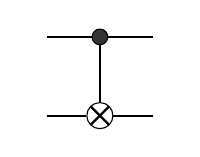
\begin{tikzpicture}[node distance=0.2cm]

\node[GHZ] (G) at (0, 0) {};
\foreach \i in {0, 2}
  {
 \pgfmathsetmacro{\ang}{90*\i}
 \pgfmathsetmacro{\x}{cos(\ang)}
 \pgfmathsetmacro{\y}{sin(\ang)}
 \node (g\i) at ($ (G)+(0.8*\x, 0.8*\y) $) {};
  \draw[thick] (G) -- (g\i);
 }

\node[circlewc] (X) at (0, -1) {};
\foreach \i in {0, 2}
  {
 \pgfmathsetmacro{\ang}{90*\i}
 \pgfmathsetmacro{\x}{cos(\ang)}
 \pgfmathsetmacro{\y}{sin(\ang)}
 \node (x\i) at ($ (X)+(0.8*\x, 0.8*\y) $) {};
  \draw[thick] (X) -- (x\i);
 }
 
 \draw[thick] (G) -- (X);

 
\end{tikzpicture}
}
\end{frame}

\begin{frame}
\scalebox{1}{
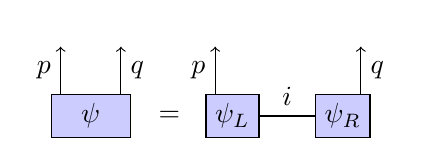
\begin{tikzpicture}[node distance=0.6cm]
\node[side, minimum width=1cm] (psi) at (0,0) {$\psi$};
\node[above=of psi.north west, anchor=south west] (p) {};
\node[above=of psi.north east, anchor=south east] (q) {};
 \draw[->] (psi.north -| p) -- node[left] {$p$} (p);
 \draw[->] (psi.north -| q) -- node[right] {$q$} (q);
 
 \node at (1, 0) {=};
 
 \node[side] (psiL) at (1.8,0) {$\psi_L$};
  \node[side] (psiR) at (3.2,0) {$\psi_R$};
\node[above=of psiL.north west, anchor=south west] (pL) {};
\node[above=of psiR.north east, anchor=south east] (qR) {};
 \draw[->] (psiL.north -| pL) -- node[left] {$p$} (pL);
 \draw[->] (psiR.north -| qR) -- node[right] {$q$} (qR);
 \draw[thick] (psiL) -- node[above] {$i$}(psiR);
 
\end{tikzpicture}

% http://hugoideler.com/2013/01/tikz-node-positioning/
% \begin{tikzpicture}[
  % every node/.style={draw, minimum size=1cm, thick, fill=white, rounded corners},
  % hi/.style={fill=red!50},
  % low/.style={fill=blue!50},
% ]
  % \node[low, minimum width=5cm] (basis) {};
  % \node[hi, above=of basis.north west, anchor=south west] (a) {A};
  % \node[hi, above=of basis] (b) {B};
  % \node[hi, above=of basis.north east, anchor=south east] (c) {C};

  % \draw[->] (basis.north -| a) -- (a);
  % \draw[->] (basis) -- (b);
  % \draw[->] (basis.north -| c) -- (c);

  % \end{tikzpicture}}
\end{frame}

\begin{frame}
\scalebox{1}{
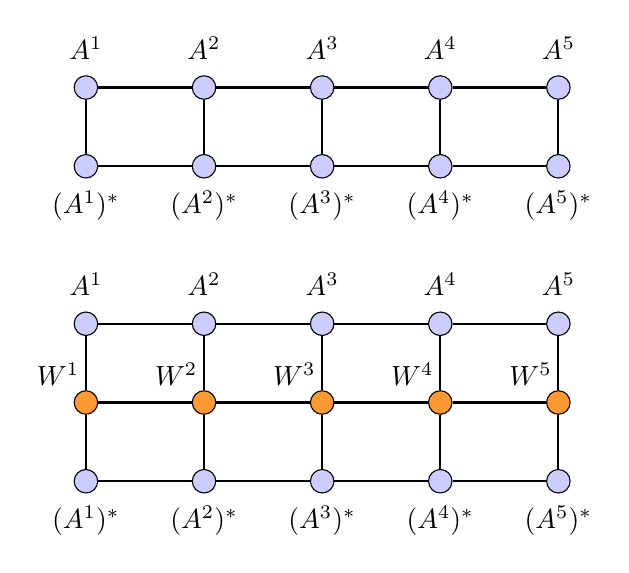
\begin{tikzpicture}[node distance=0.5cm]

\foreach \i in {1,...,5} {
	\node (Gp\i) at (1.5*\i,-2.5) [gamma] {};
	\node (Gpp\i) at ($ (Gp\i) + (0,-1) $) [gamma] {};
	\draw[thick] (Gp\i) -- (Gpp\i);
	\node[above of=Gp\i] {$A^\i$};
	\node[below of=Gpp\i] {$(A^\i)^*$};
}
\foreach \i / \j in {1/2,2/3,3/4,4/5} {
	\draw[thick] (Gp\i) -- (Gp\j);
	\draw[thick] (Gpp\i) -- (Gpp\j);
}

\foreach \i in {1,...,5} {
	\node (Gp\i) at (1.5*\i,-5.5) [gamma] {};
	\node (Gpp\i) at ($ (Gp\i) + (0,-2) $) [gamma] {};
	\node (O\i) at ($ (Gp\i) + (-0,-1) $) [operator] {};
	
	\draw[thick] (Gp\i) -- (O\i);
	\draw[thick] (Gpp\i) -- (O\i);
	
	\node[above of=Gp\i] {$A^\i$};
	\node[below of=Gpp\i] {$(A^\i)^*$};
	\node[above left of=O\i] {$W^\i$};
}
\foreach \i / \j in {1/2,2/3,3/4,4/5} {
	\draw[thick] (Gp\i) -- (Gp\j);
	\draw[thick] (Gpp\i) -- (Gpp\j);
	\draw[thick] (O\i) -- (O\j);
}

\end{tikzpicture}
}
\end{frame}

\begin{frame}
\scalebox{1}{
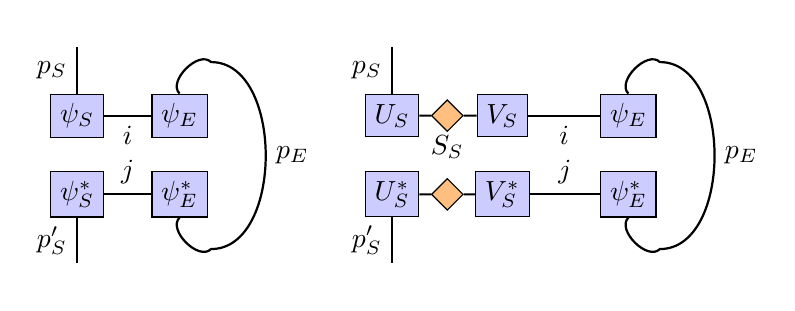
\begin{tikzpicture}[node distance=0.6cm]
\node[side] (kL) at (0,0) {$\psi_S$};
\node[side] (kR) at (1.3, 0) {$\psi_E$};
\draw[thick] (kL) -- node[below] {$i$} (kR);
\node (kLp) at (0, 1) {};
\draw[thick] (kL) -- node[left] {$p_S$} (kLp);

\node[side] (bL) at (0,-1) {$\psi_S^*$};
\node[side] (bR) at (1.3, -1) {$\psi_E^*$};
\draw[thick] (bL) -- node[above] {$j$} (bR);
\node (bLp) at (0, -2) {};
\draw[thick] (bL) -- node[left] {$p'_S$} (bLp);

\node (kRp) at ($(kR.north)+(0.4, 0.4)$) {};
\node (bRp) at ($(bR.south)+(0.4, -0.4)$) {};
\draw[thick] (kR.north) to [bend left= 90] (kRp.center) to  [bend left=90] node[right] {$p_E$}  (bRp.center) to [bend left=90] (bR.south);


\node[side] (UL) at (4, 0) {$U_S$};
\node[side] (VL) at (5.4, 0) {$V_S$};
\node[lambda] (SL) at (4.7, 0) {};
%\node[bel0w of=S] {$S_S$};

\draw[thick] (UL) -- (SL) -- (VL);
%\node[side] (kL) at (4,0) {$\psi_S$};
\node[side] (kR) at (7, 0) {$\psi_E$};
\draw[thick] (VL) -- node[below] {$i$} (kR);
\node (kLp) at (4, 1) {};
\draw[thick] (UL) -- node[left] {$p_S$} (kLp);


\node[side] (UdL) at (4, -1) {$U_S^*$};
\node[side] (VdL) at (5.4, -1) {$V_S^*$};
\node[lambda] (SdL) at (4.7, -1) {};
\node[above of=SdL] {$S_S$};

\draw[thick] (UdL) -- (SdL) -- (VdL);
\node[side] (bR) at (7, -1) {$\psi_E^*$};
\draw[thick] (VdL) -- node[above] {$j$} (bR);
\node (bLp) at (4, -2) {};
\draw[thick] (UdL) -- node[left] {$p'_S$} (bLp);

\node (kRp) at ($(kR.north)+(0.4, 0.4)$) {};
\node (bRp) at ($(bR.south)+(0.4, -0.4)$) {};
\draw[thick] (kR.north) to [bend left= 90] (kRp.center) to  [bend left=90] node[right] {$p_E$}  (bRp.center) to [bend left=90] (bR.south);


\end{tikzpicture}}
\end{frame}

\begin{frame}
\begin{columns}
\begin{column}{0.33\textwidth}
\scalebox{0.4}{
 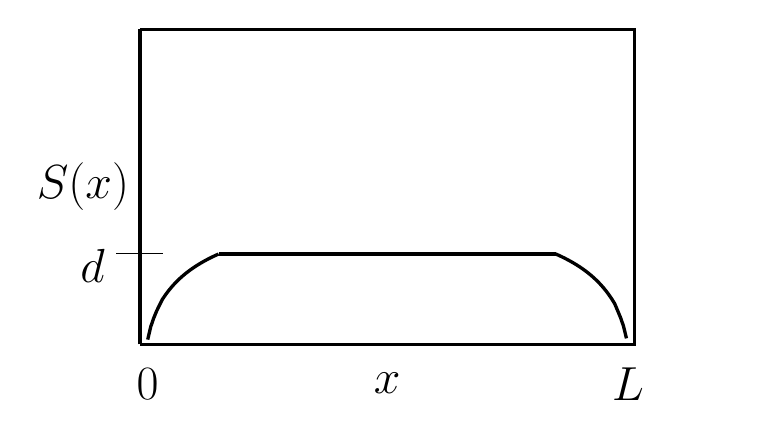
\begin{tikzpicture}[domain=0.1:6.18]
      \draw[very thick] (0, 0) -- (0,4) node[left, midway] {\LARGE $S(x)$} ;
     \node[] at (7.5, 2) {$$};
      \node[] at (3.14, -0.5){\LARGE $x$};
      \node[] at (-0.6, 1){\LARGE $d$};
      \draw[] (-0.3, 1.15) -- (0.3, 1.15);
       \node[] at (0.1, -0.5){\LARGE $0$};
       \node[] at (6.2, -0.5){\LARGE $L$};
      % \draw[thick] (0, 3.05) -- (3.14, 3.05);
      \draw[very thick] (0, 4)-- (6.28,4) -- (6.28, 0) -- (0, 0);
      \draw[color=black, very thick, domain=0.1:1] plot (\x,{1.5+1/3*log2(sin(\x/2 r))}) node[right] {};
	\draw[color=black, very thick, domain=1:5.28] plot (\x,{1.5+1/3*log2(sin(1/2 r))}) node[right] {};
	\draw[color=black, very thick, domain=5.28:6.18] plot (\x,{1.5+1/3*log2(sin(\x/2 r))}) node[right] {};
\end{tikzpicture}}
\end{column}
\begin{column}{0.33\textwidth}
\scalebox{0.4}{
 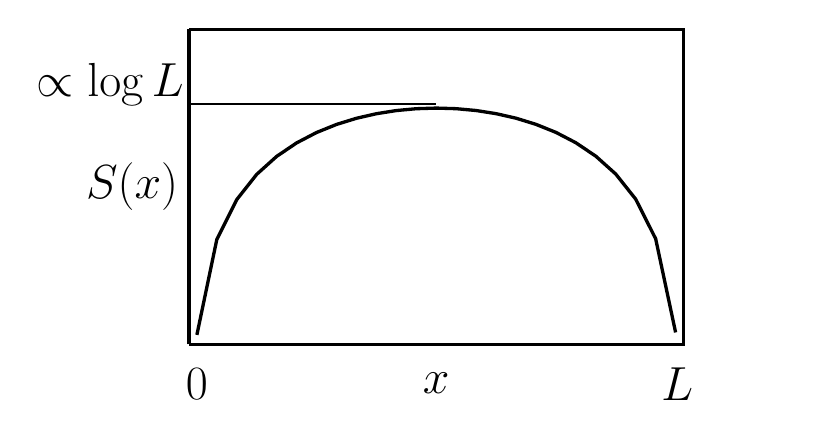
\begin{tikzpicture}[domain=0.1:6.18]
      \draw[very thick] (0, 0) -- (0,4) node[left, midway] {\LARGE $S(x)$} ;
       \node[] at (7.5, 2) {$$};
      \node[] at (3.14, -0.5){\LARGE $x$};
       \node[] at (-1, 3.3){\LARGE $\propto \log{L}$};
       \node[] at (0.1, -0.5){\LARGE $0$};
       \node[] at (6.2, -0.5){\LARGE $L$};
       \draw[thick] (0, 3.05) -- (3.14, 3.05);
      \draw[very thick] (0, 4)-- (6.28,4) -- (6.28, 0) -- (0, 0);
            \draw[color=black, very thick] plot (\x,{3+2/3*log2(sin(\x/2 r))}) node[right] {};
  \end{tikzpicture}}
\end{column}
\begin{column}{0.33\textwidth}
\scalebox{0.4}{
 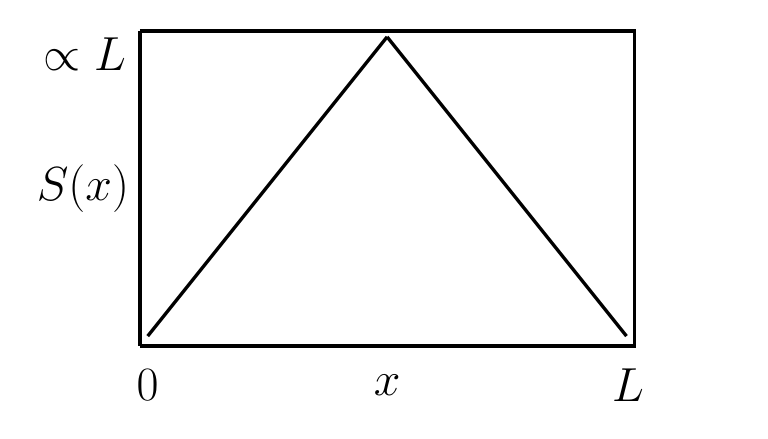
\begin{tikzpicture}[domain=0.1:6.18]
      \draw[very thick] (0, 0) -- (0,4) node[left, midway] {\LARGE $S(x)$} ;
       \node[] at (7.5, 2) {$$};
      \node[] at (3.14, -0.5){\LARGE $x$};
      \node[] at (0.1, -0.5){\LARGE $0$};
      \node[] at (6.2, -0.5){\LARGE $L$};
      \node[] at (-0.7, 3.7){\LARGE $\propto L$};
      \draw[very thick] (0, 4)-- (6.28,4) -- (6.28, 0) -- (0, 0);
      \draw[color=black, very thick, domain=0.1:3.14] plot (\x,{1.25*\x}) node[right] {};
      \draw[color=black, very thick, domain=3.14:6.18] plot (\x,{1.25*(6.28 - \x)}) node[right] {};
  \end{tikzpicture}}
\end{column}
\end{columns}
\end{frame}

\begin{frame}
\scalebox{1}{
\input{diagrams/fbi1.tex}}
\end{frame}

\begin{frame}
\scalebox{1}{
\input{diagrams/fbi2.tex}}
\end{frame}

\begin{frame}
\scalebox{1}{
% y=\sqrt{3/4}*(minimum size)/2
%

%http://tex.stackexchange.com/questions/6019/drawing-hexagons
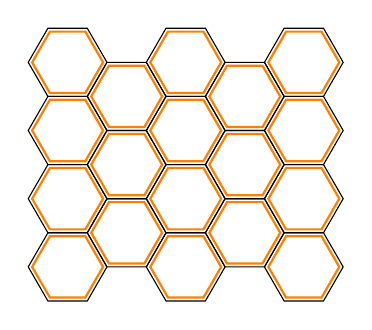
\begin{tikzpicture}[x=7.5mm,y=4.33mm]
  % some styles
  \tikzset{
    box/.style={
      regular polygon,
      regular polygon sides=6,
      minimum size=10mm,
      inner sep=0mm,
      outer sep=0mm,
      rotate=0,
     %dotted,
     thin,
      black,
      draw
    }
  }
  \tikzset{
    bbox/.style={
      regular polygon,
      regular polygon sides=6,
      minimum size=9mm,
      inner sep=0mm,
      outer sep=0mm,
      rotate=0,
     % dotted,
     thick,
     orange,
      draw
    }
  }
 \tikzset{boson/.style={circle=1pt,draw=black!100,fill=orange!100,inner sep=2pt}}
  \tikzset{dimer/.style={ellipse=1pt,draw=black!100,fill=orange!90,inner sep=2pt}}
    \tikzset{thindimer/.style={ellipse=1pt,draw=black!100,fill=orange!90,inner sep=1pt}}

\foreach \i in {0,...,2} 
    \foreach \j in {0,...,3} {
            \node[box] at (2*\i,2*\j) {};
        }
\foreach \i in {0,...,1} 
    \foreach \j in {0,...,2} {
   	   \node[box] at (2*\i+1,2*\j+1) {};   
        }
        
\foreach \i in {0,...,2} 
    \foreach \j in {0,...,3} {
            \node[bbox] at (2*\i,2*\j) {};
        }
\foreach \i in {0,...,1} 
    \foreach \j in {0,...,2} {
   	   \node[bbox] at (2*\i+1,2*\j+1) {};   
        }

\end{tikzpicture}}
\end{frame}

\begin{frame}
\scalebox{1}{
\input{diagrams/FI_PEPS_cut.tex}}
\end{frame}

\begin{frame}
\scalebox{1}{
 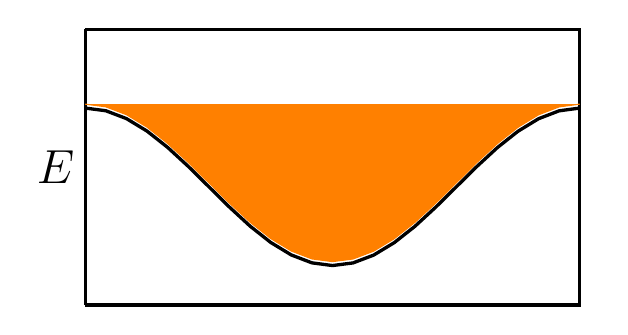
\begin{tikzpicture}[domain=0:6.28]
      \draw[very thick] (0, -2.5) -- (0,1) node[left, midway] {\LARGE $E$} ;
      \draw[very thick] (0, 1)-- (6.28,1) -- (6.28, -2.5) -- (0, -2.5);
      \draw[color=black, very thick] plot (\x,{-1+cos(\x r)}) node[right] {};
      \draw[color=orange, fill] plot (\x,{-0.95+cos(\x r)}) {};
  \end{tikzpicture}
  }
\end{frame}

\begin{frame}
\scalebox{1}{
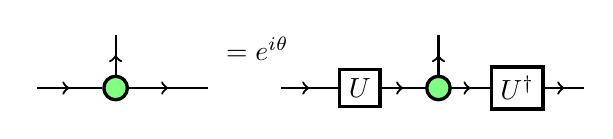
\begin{tikzpicture}
\begin{scope}[very thick,decoration={
    markings,
    mark=at position 0.5 with {\arrow{>}}}
    ] 

\node[peps] (A1) at (-4.1, 0) {};
\node (li) at ($(A1) + (-1, 0) $) {};
\draw[thick, postaction={decorate}] (li.center) -- (A1.west);
\draw[thick, postaction={decorate}] (A1.east) -- node[right] {} +(1,0);
\draw[thick, postaction={decorate}] (A1.north) -- node[above] {} +(0,0.5);

\node at (-2.3, 0.5){$= e^{i \theta}$};    

\node[peps] (A) at (0, 0) {};
\node[draw] (Ul) at ($(A) + (-1, 0) $) {$U$};
\node[draw] (Ur) at ($(A) + (1, 0) $) {$U^{\dagger}$};
\node (LI) at ($(Ul) + (-1, 0) $) {};
\draw[thick, postaction={decorate}] (LI.center) -- (Ul.west);
\draw[thick, postaction={decorate}] (Ur.east) -- node[right] {} +(0.5,0);
\draw[thick, postaction={decorate}] (Ul) -- (A);
\draw[thick, postaction={decorate}] (A) -- (Ur);
\draw[thick, postaction={decorate}] (A.north) -- node[above] {} +(0,0.5);

\end{scope}
\end{tikzpicture}}
\end{frame}

\begin{frame}
\scalebox{1}{

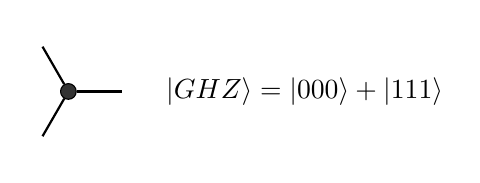
\begin{tikzpicture}[node distance=0.2cm]

\node[GHZ] (G) at (0, 0) {};
\foreach \i in {1, 2, 3}
  {
 \pgfmathsetmacro{\ang}{120*\i}
 \pgfmathsetmacro{\x}{cos(\ang)}
 \pgfmathsetmacro{\y}{sin(\ang)}
 \node (g\i) at ($ (G)+(0.8*\x, 0.8*\y) $) {};
  \draw[thick] (G) -- (g\i);
 }

 
 
 \node at (3, 0) {$\ket{GHZ} = \ket{000}+\ket{111}$};

 
\end{tikzpicture}}
\end{frame}

\begin{frame}
\scalebox{1}{
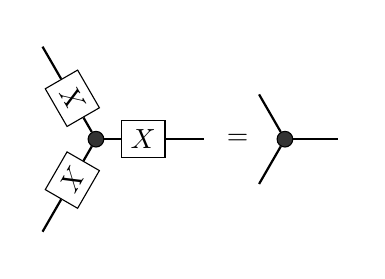
\begin{tikzpicture}[node distance=0.2cm]

\node[GHZ] (G) at (0, -2) {};
\foreach \i in {1, 2, 3}
  {
 \pgfmathsetmacro{\ang}{120*\i}
 \pgfmathsetmacro{\x}{cos(\ang)}
 \pgfmathsetmacro{\y}{sin(\ang)}
 \node[draw, rotate=\ang] (gx\i) at ($ (G)+(0.6*\x, 0.6*\y) $) {$X$};
 \node[inv] (g\i) at ($ (G)+(1.5*\x, 1.5*\y) $) {};
 }
 
\foreach \i in {1, 2, 3}
  {
 \draw[thick] (G) -- (gx\i) --(g\i);
 } 
 
\node at (1.8, -2) {$=$};

\node[GHZ] (G3) at (2.4, -2) {};
\foreach \i in {1, 2, 3}
  {
 \pgfmathsetmacro{\ang}{120*\i}
 \pgfmathsetmacro{\x}{cos(\ang)}
 \pgfmathsetmacro{\y}{sin(\ang)}
 \node (g\i) at ($ (G3)+(0.8*\x, 0.8*\y) $) {};
 }
 \foreach \i in {1, 2, 3}
  {
 \draw[thick] (G3) -- (g\i);
 }

\end{tikzpicture}}
\end{frame}

\begin{frame}
\scalebox{1}{
\input{diagrams/honeycomb3.tex}}
\end{frame}

\begin{frame}
\scalebox{1}{
%
% x=3*(minimum size)/2
% y=\sqrt{3/4}*(minimum size)/2
%

%http://tex.stackexchange.com/questions/6019/drawing-hexagons
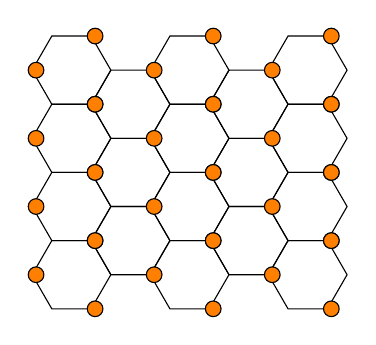
\begin{tikzpicture}[x=7.5mm,y=4.33mm]
  % some styles
  \tikzset{
    box/.style={
      regular polygon,
      regular polygon sides=6,
      minimum size=10mm,
      inner sep=0mm,
      outer sep=0mm,
      rotate=0,
    draw
    }
  }
 \tikzset{boson/.style={circle=1pt,draw=black!100,fill=orange!100,inner sep=2pt}}

\foreach \i in {0,...,2} 
    \foreach \j in {0,...,3} {
            \node[box] at (2*\i,2*\j) {};
        }
\foreach \i in {0,...,1} 
    \foreach \j in {0,...,2} {
   	   \node[box] at (2*\i+1,2*\j+1) {};   
        }
\foreach \i in {0,...,2} 
    \foreach \j in {0,...,3} {
            \node[boson] at (2*\i-0.6,2*\j) {};
           % \node[boson] at (2*\i+0.6,2*\j) {};
           % \node[boson] at (2*\i-0.4,2*\j-1) {};
           % \node[boson] at (2*\i-0.4,2*\j+1) {};
             \node[boson] at (2*\i+0.4,2*\j+1) {};
              \node[boson] at (2*\i+0.4,2*\j-1) {};
        }
%\foreach \i in {0,...,1} 
  %  \foreach \j in {0,...,2} {
%	\node[boson] at (2*\i+1-0.6,2*\j+1) {}; 
%	\node[boson] at (2*\i+1+0.6,2*\j+1) {};   
   %   }
      
\end{tikzpicture}
}
\end{frame}

\begin{frame}
\scalebox{1}{
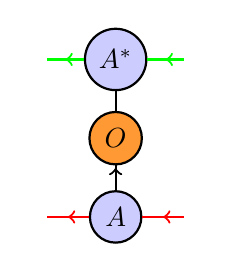
\begin{tikzpicture}[node distance=0.4cm]
\begin{scope}[thick, decoration={
    markings,
    mark=at position 0.5 with {\arrow{>}}}
    ]
  \node[gamma] (A) at (0,0) {$A$};  
  \node[operator] (O) at (0, 1) {$O$};
 % \node[operator] (O2) at (0, 1) {$O'$};
  \node[gamma] (Ac) at (0,2) {$A^{*}$};
  \draw[postaction={decorate}] (A)-- (O) -- (Ac);
  \node[inv] (ki) at (1, 0){};
  \node[inv] (bi) at (1, 2){}; 
  \node[inv] (ko) at (-1, 0){}; 
  \node[inv] (bo) at (-1, 2){};
  \draw[color=red, postaction={decorate}] (ki)--(A);
  \draw[color=green, postaction={decorate}] (bi)--(Ac);
  \draw[color=red, postaction={decorate}] (A) -- (ko);
  \draw[color=green, postaction={decorate}] (Ac) -- (bo);

\end{scope}
\end{tikzpicture}}
\end{frame}

\begin{frame}
\scalebox{1}{
%
% x=3*(minimum size)/2
% y=\sqrt{3/4}*(minimum size)/2
%

%http://tex.stackexchange.com/questions/6019/drawing-hexagons
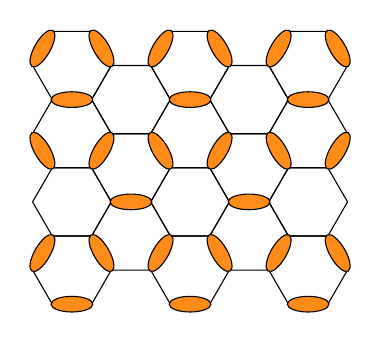
\begin{tikzpicture}[x=7.5mm,y=4.33mm]
  % some styles
  \tikzset{
    box/.style={
      regular polygon,
      regular polygon sides=6,
      minimum size=10mm,
      inner sep=0mm,
      outer sep=0mm,
      rotate=0,
    draw
    }
  }
 \tikzset{boson/.style={circle=1pt,draw=black!100,fill=orange!100,inner sep=2pt}}
  \tikzset{dimer/.style={ellipse=1pt,draw=black!100,fill=orange!90,inner sep=2pt}}

\foreach \i in {0,...,2} 
    \foreach \j in {0,...,3} {
            \node[box] at (2*\i,2*\j) {};
        }
\foreach \i in {0,...,1} 
    \foreach \j in {0,...,2} {
   	   \node[box] at (2*\i+1,2*\j+1) {};   
        }
% \foreach \i in {0,...,2} 
%     \foreach \j in {0,...,3} {
%     	  %\node[boson] at (2*\i-0.4,2*\j+1) {}; %TL of A hexagon
%          %\node[boson] at (2*\i+0.6,2*\j) {}; %R of A hexagon
%          %\node[boson] at (2*\i-0.4,2*\j-1) {}; %BL of A hexagon
% 
%          %\node[boson] at (2*\i-0.6,2*\j) {}; %L of  A hexagon
%          %\node[boson] at (2*\i+0.4,2*\j+1) {}; %TR of A hexagon
%          %\node[boson] at (2*\i+0.4,2*\j-1) {}; %BR of A hexagon
%         }
% \foreach \i in {0,...,1} 
%     \foreach \j in {0,...,2} {
% %	\node[boson] at (2*\i+1-0.6,2*\j+1) {}; %L of B hexagon
% %	\node[boson] at (2*\i+1+0.6,2*\j+1) {};   %R of B hexagon
%       }
 \foreach \i in {-1,...,2} 
     \foreach \j in {0,...,2} 
     {
     \pgfmathtruncatemacro{\x}{2*\i + 1*\j}
     \pgfmathtruncatemacro{\y}{3*\j}
     \ifnum
     -1<\x
     \ifnum
     \x<5
     \ifnum
     \y<7
     \ifnum
     -1<\y     
     \node[dimer, rotate=120] at (\x+1/2,\y+1/2) {$\,\,\,\,$};
     \node[dimer, rotate=60] at (\x-1/2,\y+1/2) {$\,\,\,\,$};
     \node[dimer, rotate=0] at (\x,\y-1) {$\,\,\,\,$};
     \fi
     \fi
     \fi
     \fi
     %\node[boson] at (\x, \y) {}; 
     }
    \node[dimer, rotate=120] at (0-1/2,3+1/2) {$\,\,\,\,$};
    \node[dimer, rotate=60] at (5-1/2,3+1/2) {$\,\,\,\,$};
      
\end{tikzpicture}}
\end{frame}

\begin{frame}
\scalebox{1}{
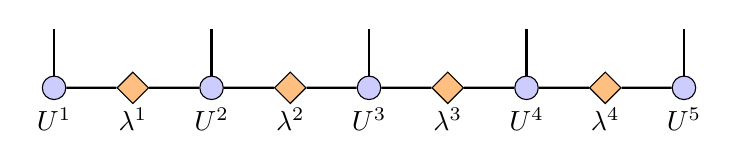
\begin{tikzpicture}[node distance=0.4cm]

\foreach \i / \j in {1/A,2/B,3/A,4/B,5/A}
{
	\node[gamma] (G\i) at (2*\i-2,2.5) {};
	\node[below of=G\i] {$U^\i$};
	\draw[thick] (G\i) -- ($ (G\i) + (0, 0.75) $);
}
\foreach \i / \j in {1/A, 2/B,3/A,4/B}
{
	\node[lambda] (l\i) at (2*\i-1,2.5) {};
	\node[below of=l\i] {$\lambda^\i$};
}

\foreach \i / \j in {1/2,2/3,3/4,4/5}
{
	\draw[thick] (l\i) -- (G\i);
	\draw[thick] (l\i) -- (G\j);
}

%\draw[thick,dashed] (l1) -- ($ (l1) + (-0.5,0) $);
%\draw[thick,dashed] (l6) -- ($ (l6) + (0.5,0) $);

\end{tikzpicture}}
\end{frame}

\begin{frame}
\scalebox{1}{
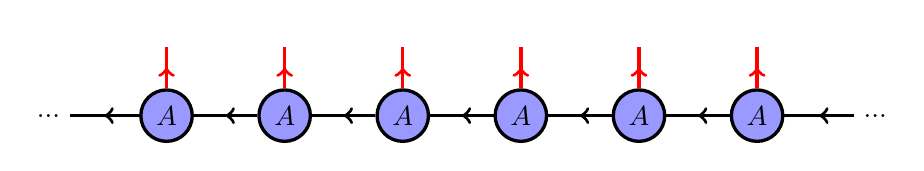
\begin{tikzpicture}[node distance=0.4cm]
\tikzset{gamma/.style={circle=2pt,draw=black!100, very thick, fill=blue!40, inner sep=3pt}}


\begin{scope}[decoration={
    markings,
    mark=at position 0.5 with {\arrow{>}}}
    ]

\foreach \i in {1,...,6} {
	\node[gamma] (G\i) at (1.5*\i,0) {$A$};
	\node (l\i) at ($ (G\i) + (0, 1) $) {$$};
	\draw[very thick, red!100, postaction={decorate}] (G\i) -- (l\i);
	%\node[below of=G\i] {$A$};
}

\foreach \i in {7} {
	\node[] (G\i) at (1.5*\i,0) {$...$};
    }  
    
\foreach \i / \j in {1/2,2/3,3/4,4/5,5/6, 6/7} {
	\draw[very thick, postaction={decorate}] (G\j) -- (G\i);
}
\node (b0) at (0, 0) {$...$};
\draw[very thick, postaction={decorate}] (G1) -- (b0);

\end{scope}
\end{tikzpicture}
}
\end{frame}

\begin{frame}
\scalebox{1}{
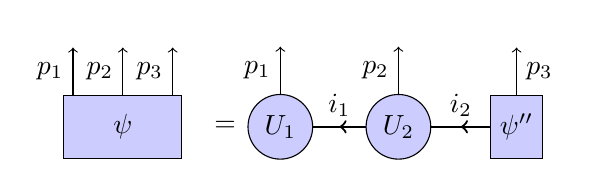
\begin{tikzpicture}[node distance=0.6cm]
    \node[side, minimum width=1.5cm, minimum height=0.8cm] (psi) at (0,0) {$\psi$};
    \node[above=of psi.north west, anchor=south west] (p1) {};
    \node[above=of psi](p2) {};
    \node[above=of psi.north east, anchor=south east] (p3) {};
    \node at (1.3, 0) {=};
    \node[cside] (B1) at (2,0) {$U_1$};
    \node[cside] (B2) at (3.5,0) {$U_2$};
    \node[side, minimum width=0.5cm, minimum height=0.8cm](psiR) at (5, 0){$\psi''$};
    %\node[lambda] (S) at (3, 0) {};
    %\node[side,minimum width=1cm, minimum height=0.8cm] (psiR) at (4.2,0) {$\psi'$};
    \node[above=of B1.north, anchor=south] (pL) {};
    \node[above=of B2] (q2) {};
    %\node[above=of psiR.north west, anchor=south west] (q2) {};
    \node[above=of psiR.north, anchor=south] (qR) {};
\begin{scope}[decoration={
    markings,
    mark=at position 0.5 with {\arrow{>}}}
    ]
    \draw[->] (psi.north -| p1) -- node[left] {$p_1$} (p1);
    \draw[->] (psi) --  node[left] {$p_2$} (p2);
    \draw[->] (psi.north -| p3) -- node[left] {$p_3$} (p3);
    \draw[->] (B1.north -| pL) -- node[left] {$p_1$} (pL);
    \draw[->] (B2.north-|q2)-- node[left] {$p_2$} (q2);
    \draw[->] (psiR.north -| qR) -- node[right] {$p_3$} (qR);
    \draw[-, thick, postaction={decorate}] (B2) -- node[above]{$i_1$}(B1);
    \draw[-, thick, postaction={decorate}] (psiR) -- node[above]{$i_2$}(B2);
 %\draw[-] (psiR) -- (S);
  \end{scope}
\end{tikzpicture}}
\end{frame}

\begin{frame}
\scalebox{1}{
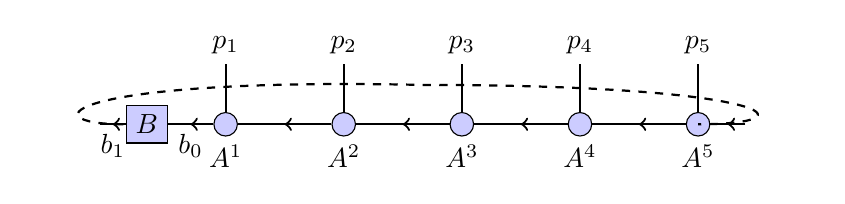
\begin{tikzpicture}[node distance=0.4cm]
\begin{scope}[decoration={
    markings,
    mark=at position 0.5 with {\arrow{>}}}
    ]
\foreach \i in {1,...,5} {
	\node[gamma] (G\i) at (1.5*\i,0) {};
	\node (l\i) at ($ (G\i) + (0, 1) $) {$p_\i$};
	\draw[thick] (G\i) -- (l\i);
	\node[below of=G\i] {$A^\i$};
}
\foreach \i / \j in {1/2,2/3,3/4,4/5} {
	\draw[thick, postaction={decorate}] (G\j) -- (G\i);
}
\node[side] (B) at (0.5, 0) {$B$};
%\node (b1) at (0, 0) {$b_1$};
\draw[thick, postaction={decorate}] (G1) -- node[below]{$b_0$}(B);
\draw[thick, postaction={decorate}] (8.1, 0)--(G5.east);
\draw[thick, postaction={decorate}] (B.west) -- node[below]{$b_1$}(-0.1, 0);
\end{scope}
\draw[thick, dashed] (0.2,0) .. controls (-1,0) and (-0.6,0.6) .. (4,0.5) .. controls (8.5,0.5) and (9,0) .. (7.5,0);
\end{tikzpicture}}
\end{frame}

\begin{frame}
\scalebox{1}{
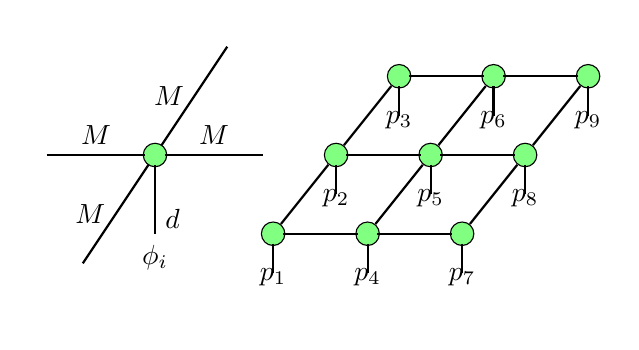
\begin{tikzpicture}
\foreach \i in {1,...,3}
\foreach \j in {2}
{ {
	\node (G\i\j) at (1.5*\i+1*\j,1.5*\j) {};
} }

\foreach \i in {2}
\foreach \j in {1, 3}
{ {
	\node (G\i\j) at (1.5*\i+1*\j,1.5*\j) {};
} }

\foreach \k / \i in {1/2}
\foreach \l / \j in {1/2}
{ {
	\node at (G\i\j) [peps] {};
	\draw[thick] (G\i\j) -- node[below right ] {$d$} +(0,-1);
	\node at ($ (G\i\j)+(0,-1.3) $) {$\phi_i$};
} }
\foreach \i in {2}
\foreach \j / \l in {1/2,2/3}
{ {
	\draw[thick] (G\i\j) -- node[left] {$M$} (G\i\l);
	\draw[thick] (G\j\i) -- node[above] {$M$} (G\l\i);
} }

\foreach \i in {1,...,4}
\foreach \j in {1,...,4}
{ {
	\node (G\i\j) at (2.5+1.2*\i+0.8*\j,1*\j) [inv] {};
} }

\foreach \i / \j / \k in {2/2/1,2/3/2,2/4/3,3/2/4,3/3/5,3/4/6,4/2/7,4/3/8,4/4/9}
{
	\node at (G\i\j) [peps] {};
	\draw[thick] (G\i\j) -- node[below] {$p_{\k}$} +(0,-0.5);
}
\foreach \i in {2,3,4}
\foreach \j / \l in {2/3,3/4}
{ {
	\draw[thick] (G\i\j) -- (G\i\l);
	\draw[thick] (G\j\i) -- (G\l\i);
} }
\end{tikzpicture}}
\end{frame}

\begin{frame}
\scalebox{1}{
\input{diagrams/productstate.tex}}
\end{frame}

\begin{frame}
\scalebox{1}{
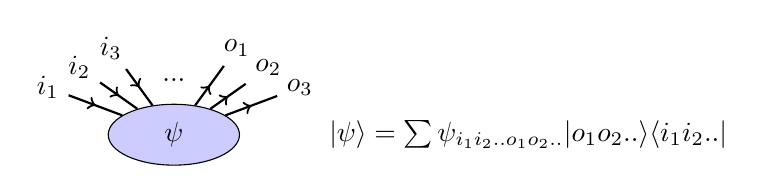
\begin{tikzpicture}[node distance=0.4cm]]
\tikzset{det/.style={circle=2pt,fill=blue!20,draw=black,inner sep=4pt}}
\node[ellipse, rotate=0, draw, fill=blue!20] (t) at (0,0) {\, \, $\psi$ \, \,};
\node (t1) at (-1.6, 0.6) {$i_1$};
\node (t2) at (-1.2 ,0.85) {$i_2$};
\node (t3) at (-0.8,1.1) {$i_3$};
\node (o3) at (1.6, 0.6) {$o_3$};
\node (o2) at (1.2 ,0.85) {$o_2$};
\node (o1) at (0.8,1.1) {$o_1$};
\node[rotate=0] (d) at (0, 0.7) {...};

\begin{scope}[very thick,decoration={
    markings,
    mark=at position 0.5 with {\arrow{>}}}
    ] 
\draw[thick, postaction={decorate}] (t1) -- (t);
\draw[thick,postaction={decorate}] (t2) -- (t);
\draw[thick, postaction={decorate}] (t3) -- (t);
\draw[thick, postaction={decorate}] (t) -- (o1);
\draw[thick,postaction={decorate}] (t) -- (o2);
\draw[thick, postaction={decorate}] (t) -- (o3);
\end{scope}

\node (p) at (4.5,0) {$\ket{\psi} = \sum \psi_{i_1 i_2 .. o_1 o_2 ..} \vert o_1 o_2 .. \rangle \langle i_1 i_2 .. \vert$};

\end{tikzpicture}}
\end{frame}

\begin{frame}
\scalebox{1}{
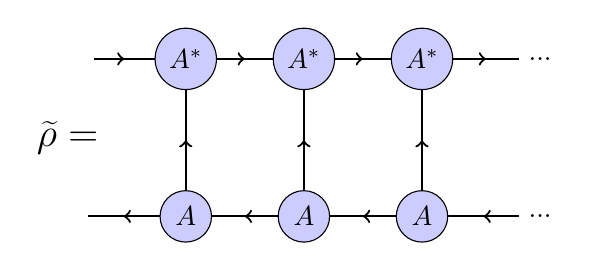
\begin{tikzpicture}[node distance=0.4cm]
\begin{scope}[decoration={
    markings,
    mark=at position 0.5 with {\arrow{>}}}
    ]
\node[] (rho) at (4.5,1) {\Large $\widetilde{\rho} =$};  

\foreach \i in {3} {
	\node[inv] (G\i) at (1.5*\i,0) {$A$};
	\node[inv] (B\i) at (1.5*\i,2) {$A^*$};
    }
\foreach \i in {7} {
	\node[] (G\i) at (1.5*\i,0) {$...$};
	\node[] (B\i) at (1.5*\i,2) {$...$};
    }    
\foreach \i in {4,...,6} {
	\node[gamma] (G\i) at (1.5*\i,0) {$A$};
	\node[gamma] (B\i) at (1.5*\i,2) {$A^*$};
	\draw[thick, postaction={decorate}] (G\i) -- (B\i);
	}
\foreach \i / \j in {3/4,4/5,5/6, 6/7} {
	\draw[thick, postaction={decorate}] (G\j) -- (G\i);
	\draw[thick, postaction={decorate}] (B\i) -- (B\j);
}
\end{scope}
\end{tikzpicture}
}
\end{frame}

\begin{frame}
\scalebox{1}{
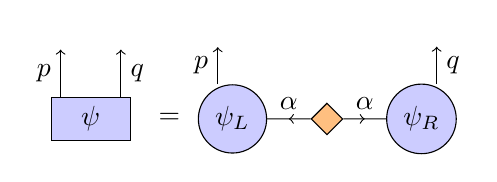
\begin{tikzpicture}[node distance=0.6cm]
\begin{scope}[decoration={
    markings,
    mark=at position 0.5 with {\arrow{>}}}
    ]
\node[side, minimum width=1cm] (psi) at (0,0) {$\psi$};
\node[above=of psi.north west, anchor=south west] (p) {};
\node[above=of psi.north east, anchor=south east] (q) {};
 \draw[->] (psi.north -| p) -- node[left] {$p$} (p);
 \draw[->] (psi.north -| q) -- node[right] {$q$} (q);
 
 \node at (1, 0) {=};
 
 \node[cside] (psiL) at (1.8,0) {$\psi_L$};
\node[lambda] (S) at (3, 0) {};
  \node[cside] (psiR) at (4.2,0) {$\psi_R$};
\node[above=of psiL.north west, anchor=south west] (pL) {};
\node[above=of psiR.north east, anchor=south east] (qR) {};
 \draw[->] (psiL.north -| pL) -- node[left] {$p$} (pL);
 \draw[->] (psiR.north -| qR) -- node[right] {$q$} (qR);
 \draw[-, postaction={decorate}] (S) -- node[above]{$\alpha$}(psiL);
 \draw[-, postaction={decorate}] (S) -- node[above]{$\alpha$}(psiR);
 
\end{scope}
\end{tikzpicture}}
\end{frame}

\begin{frame}
\scalebox{1}{
%!TEX root = ../thesis.tex

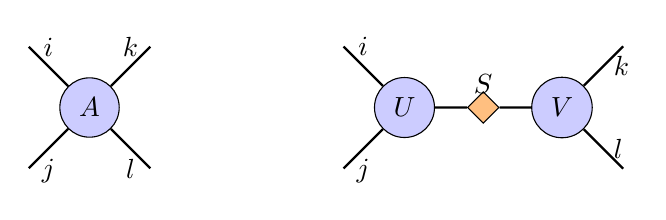
\begin{tikzpicture}

\node[det] (Ap) at (0,-0.5) {$A$};
% \node[det] (Bp) at (2,-0.5) {$B$};
% \node[det] (Cp) at (1,-2) {$C$};

% \draw[thick] (Ap.north east) -- (Bp.north west);
% \draw[thick] (Ap.south east) -- (Bp.south west);
% \draw[thick] (Ap.south) -- (Cp.north west);
% \draw[thick] (Bp.south) -- (Cp.north east);

\draw[thick] (Ap.north west) -- node[above] {$i$} +(-0.5,0.5);
\draw[thick] (Ap.south west) -- node[below] {$j$} +(-0.5,-0.5);
\draw[thick] (Ap.north east) -- node[above] {$k$} +(0.5,0.5);
\draw[thick] (Ap.south east) -- node[below] {$l$} +(0.5,-0.5);

% \draw[thick] (Cp.south) -- node[right] {$k$} +(0,-0.5);
% \draw[thick] (Bp.east) -- node[below] {$l$} +(0.5,0);

% next panel

\node[det] (U) at (4,-0.5) {$U$};
\node[det] (V) at (6,-0.5) {$V$};
\node[lambda] (S) at (5,-0.5) {};
\node[above of=S,node distance=0.3cm] {$S$};

\draw[thick] (U) -- (S) -- (V);

\draw[thick] (U.north west) -- node[above] {$i$} +(-0.5,0.5);
\draw[thick] (U.south west) -- node[below] {$j$} +(-0.5,-0.5);
\draw[thick] (V.south east) -- node[right] {$l$} +(0.5,-0.5);
\draw[thick] (V.north east) -- node[right] {$k$} +(0.5,0.5);

\end{tikzpicture}
}
\end{frame}

\begin{frame}
\scalebox{1}{
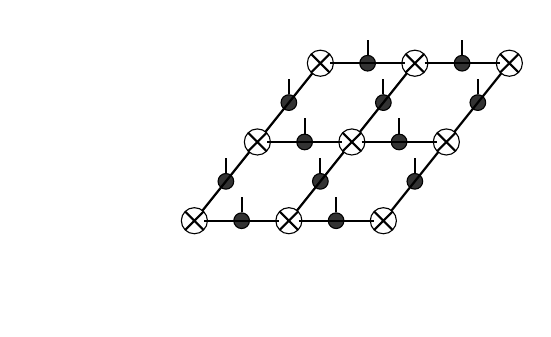
\begin{tikzpicture}
\foreach \i in {1,...,4}
\foreach \j in {1,...,4}
{ {
	\node (G\i\j) at (2.5+1.2*\i+0.8*\j,1*\j) [inv] {};
} }

\foreach \i / \j / \k in {2/2/1,2/3/2,2/4/3,3/2/4,3/3/5,3/4/6,4/2/7,4/3/8,4/4/9}
{
	\node at (G\i\j) [circlewc] {};
	%\draw[thick] (G\i\j) -- node[below] {$p_{\k}$} +(0,-0.5);
}
\foreach \i / \j / \k in {2/2/1,2/3/2,2/4/3,3/2/4,3/3/5,3/4/6}
{
	\node (HR\i\j) at ($(G\i\j)+(0.6, 0)$) [GHZ] {};
	\node (HU\j\i) at ($(G\j\i)+(0.4, 0.5)$) [GHZ] {};
	\draw[thick] (HR\i\j) -- node[above] {} +(0,0.3);
	\draw[thick] (HU\j\i) -- node[above] {} +(0,0.3);
}
\foreach \i in {2,3,4}
\foreach \j / \l in {2/3,3/4}
{ {
	\draw[thick] (G\i\j) -- (G\i\l);
	\draw[thick] (G\j\i) -- (G\l\i);
} }
\end{tikzpicture}}
\end{frame}

\begin{frame}
\scalebox{1}{

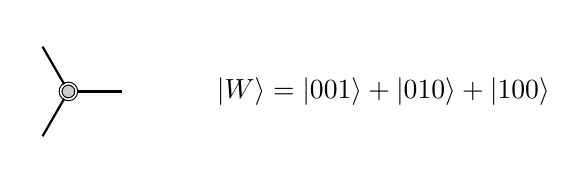
\begin{tikzpicture}[node distance=0.2cm]

\node[W] (G) at (0, 0) {};
\foreach \i in {1, 2, 3}
  {
 \pgfmathsetmacro{\ang}{120*\i}
 \pgfmathsetmacro{\x}{cos(\ang)}
 \pgfmathsetmacro{\y}{sin(\ang)}
 \node (g\i) at ($ (G)+(0.8*\x, 0.8*\y) $) {};
 }
 
\foreach \i in {1, 2, 3}
  {
 \draw[thick] (G) -- (g\i);
 } 
 
 
 \node at (4, 0) {$ \ket{W} = \ket{001}+\ket{010}+\ket{100}$};

 
\end{tikzpicture}}
\end{frame}

\begin{frame}
\scalebox{1}{
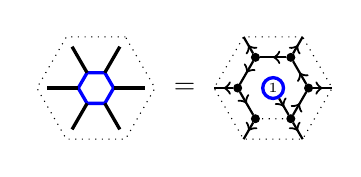
\begin{tikzpicture}[x=7.5mm,y=4.33mm]
\begin{scope}[decoration={
    markings,
    mark=at position 0.5 with {\arrow{>}}}
    ]
    
  \tikzset{
    box/.style={
      regular polygon,
      regular polygon sides=6,
      minimum size=15mm,
      inner sep=0mm,
      outer sep=0mm,
      rotate=0,
     dotted,
     thin,
      black,
      draw
    }
    }
      \tikzset{
    abox/.style={
      regular polygon,
      regular polygon sides=6,
      minimum size=9mm,
      inner sep=0mm,
      outer sep=0mm,
      rotate=0,
     dotted,
     thin,
      black,
      draw
    }
    }


    \tikzset{
    wb/.style={
       regular polygon,
      regular polygon sides=6,
      minimum size=4.5mm,
      %fill,
      inner sep=0mm,
      outer sep=0mm,
      rotate=0,
     % dotted,
     very thick,
     blue,
      draw
    }
  }
\tikzset{smalldot/.style={circle=1pt,draw=black!100,fill=black!100,inner sep=1pt}}
\tikzset{smallwdot/.style={circle=1pt, very thick, draw=blue!100,fill=white,inner sep=1pt}}

 \node[box] (H) at (0, 0) {};
\node[wb] (W) at (0,0) {};

\foreach \k in {1, ..., 6}{
             \node[inv] (D\k) at (H.corner \k) {};
             \draw[very thick, black] (W) -- (D\k);
             }
             
 \node[] at (1.5, 0){$=$};

 \node[box] (H3) at (3, 0) {};
 \node[abox] (H2) at (3, 0) {};
%\node[wb] (W) at (3,0) {\tiny W};
\foreach \k in {1, ..., 6}{
             \node[smalldot] (A\k) at (H2.corner \k) {};
             }

\foreach \k in {1,2,3,5}{
		\pgfmathtruncatemacro{\j}{\k+1}
            \draw[thick, postaction={decorate}] (A\k) -- (A\j);
             }
             \draw[thick, postaction={decorate}] (A6) -- (A1);
             
 \foreach \k in {1,2,3,4,5,6}{
            \draw[thick, postaction={decorate}] (A\k) -- (H3.corner \k);
             }
             
 \node[smallwdot](B) at (3, 0) {\tiny 1};
 \draw[thick, postaction={decorate}]  (B)--(A5);

\end{scope}
\end{tikzpicture}}
\end{frame}

\begin{frame}
\scalebox{1}{

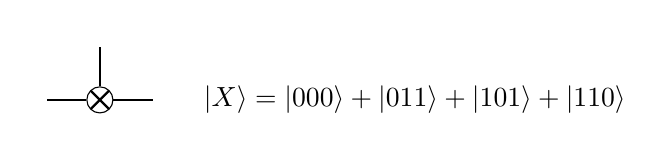
\begin{tikzpicture}[node distance=0.2cm]

\node[circlewc] (G) at (0, 0) {};
\foreach \i in {0, 1, 2}
  {
 \pgfmathsetmacro{\ang}{90*\i}
 \pgfmathsetmacro{\x}{cos(\ang)}
 \pgfmathsetmacro{\y}{sin(\ang)}
 \node (g\i) at ($ (G)+(0.8*\x, 0.8*\y) $) {};
  \draw[thick] (G) -- (g\i);
 }
 
 
 \node at (4, 0) {$\ket{X} = \ket{000}+\ket{011}+ \ket{101} + \ket{110}$};

 
\end{tikzpicture}
}
\end{frame}

\begin{frame}
\scalebox{1}{
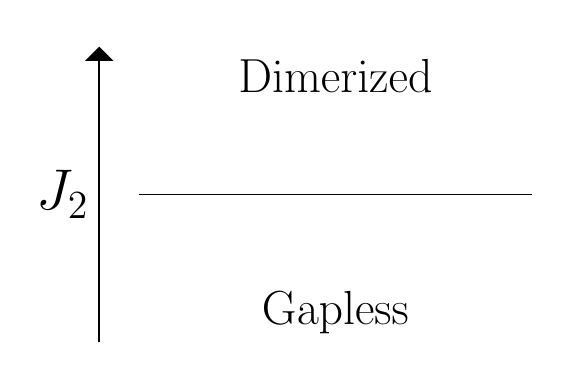
\begin{tikzpicture}
\tikzstyle{myedgestyle} = [-triangle 90]
\node[inv](A) at (0, -2){};
\node[inv](B) at (0, 2){};
\draw[thick, myedgestyle] (A)--node[left] {\huge $J_2$}(B);
\node[] at (3, -1.5){\LARGE Gapless};
\node[] at (3, 1.5){\LARGE Dimerized};
\draw[] (0.5, 0) -- (5.5, 0);
\end{tikzpicture}}
\end{frame}

\begin{frame}
\scalebox{1}{
% y=\sqrt{3/4}*(minimum size)/2
%

%http://tex.stackexchange.com/questions/6019/drawing-hexagons
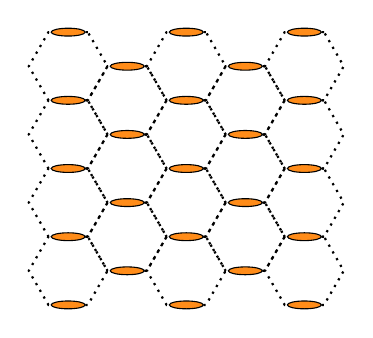
\begin{tikzpicture}[x=7.5mm,y=4.33mm]
  % some styles
  \tikzset{
    box/.style={
      regular polygon,
      regular polygon sides=6,
      minimum size=10mm,
      inner sep=0mm,
      outer sep=0mm,
      rotate=0,
      dotted,
      thick,
      black,
      draw
    }
  }
 \tikzset{boson/.style={circle=1pt,draw=black!100,fill=orange!100,inner sep=2pt}}
  \tikzset{dimer/.style={ellipse=1pt,draw=black!100,fill=orange!90,inner sep=2pt}}
    \tikzset{thindimer/.style={ellipse=1pt,draw=black!100,fill=orange!90,inner sep=1pt}}

\foreach \i in {0,...,2} 
    \foreach \j in {0,...,3} {
            \node[box] at (2*\i,2*\j) {};
        }
\foreach \i in {0,...,1} 
    \foreach \j in {0,...,2} {
   	   \node[box] at (2*\i+1,2*\j+1) {};   
        }

 \foreach \i in {-1,...,2} 
     \foreach \j in {-1,...,2} 
     {
     \pgfmathtruncatemacro{\xa}{2*\i + 1*\j}
     \pgfmathtruncatemacro{\ya}{3*\j}
      \pgfmathtruncatemacro{\xb}{2*\i + 1*\j+1}
     \pgfmathtruncatemacro{\yb}{3*\j+1}
      \pgfmathtruncatemacro{\xc}{2*\i + 1*\j}
     \pgfmathtruncatemacro{\yc}{3*\j+2}
    
    \ifnum -1<\xa \ifnum \xa<5
     \ifnum\ya<7\ifnum-1<\ya 
	% \node[thindimer, rotate=120] at (\x-1/2,\y-1/2) {$\,\,\,\,$};     
     %\node[thindimer, rotate=120] at (\x+1/2,\y+1/2) {$\,\,\,\,$};
     %\node[thindimer, rotate=60] at (\x-1/2,\y+1/2) {$\,\,\,\,$};
       %\node[thindimer, rotate=60] at (\x+1/2,\y-1/2) {$\,\,\,\,$};
     \node[thindimer, rotate=0] at (\xa,\ya-1) {$\,\,\,\,$};
      \node[thindimer, rotate=0] at (\xa,\ya+1) {$\,\,\,\,$};
     \fi \fi\fi\fi
     
      \ifnum -1<\xc\ifnum \xc<5
     \ifnum \yc<7 \ifnum -2<\yc
       \node[thindimer, rotate=0] at (\xc,\yc+1) {$\,\,\,\,$};
       \fi\fi\fi \fi 
     }

\end{tikzpicture}}
\end{frame}
\end{document}
